\documentclass[a4paper,norsk]{article}
\usepackage{preamble}

\begin{document}

\maketitle
\section*{Assignment I}
In this assignment we are tasked to implement a non-linear solver for the Falkner-Skan equation
\begin{align*}
f^{\prime\prime\prime} + ff^{\prime\prime} + \beta\Big(1-(f^{\prime2})\Big) = 0 \\
\beta = \frac{2m}{m+1}
\end{align*}
Varying the parameter $\beta$ gives the following results

\begin{figure}[h!]	
	\centering
	\caption*{Plot of the f derivative for different $\beta$ }
	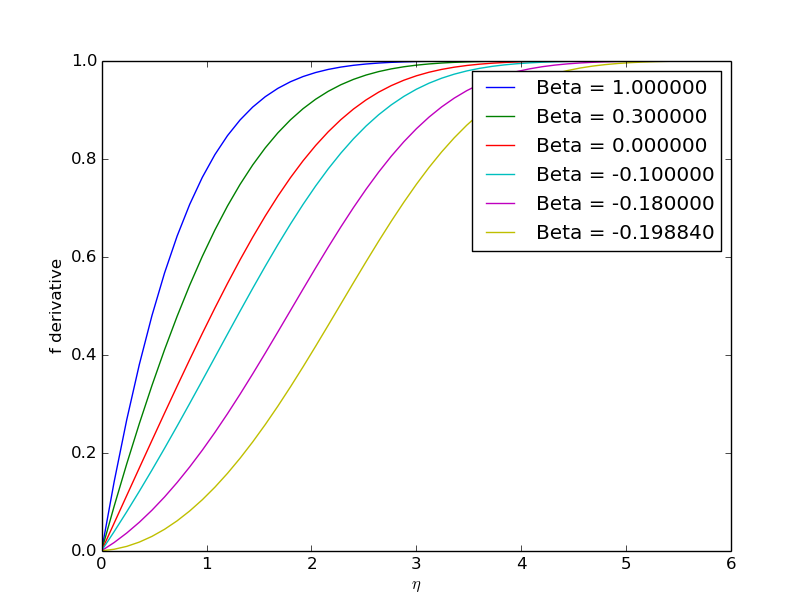
\includegraphics[scale = 0.6]{mand1/fderi.png}
\end{figure}
\begin{figure}[h!]	
	\centering
	\caption*{Plot of the h derivative for different $\beta$}
	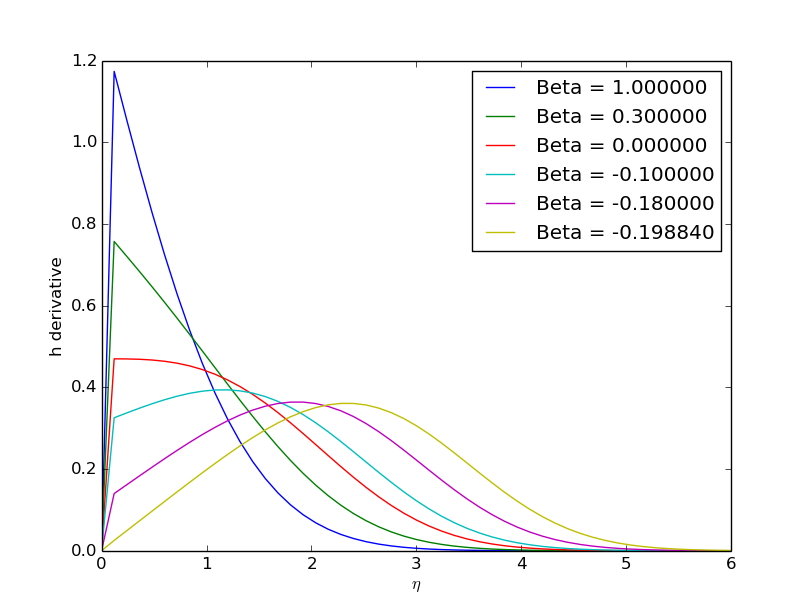
\includegraphics[scale = 0.6]{mand1/hderi.png}
\end{figure}
\newpage
For some reason my program doesn't add the second first point in the plot, making the graph take a leap to the first value. Other than that, I conclude that the program reproduces the figure 4-11 presented in White.
\newline

We are also tasked to find a solution which showes negative walues for $f^\prime (0)$. As observed in the plots, with the right guess, we get a solution as mentioned. This indicating a backflow close to the wall.
\begin{figure}[h!]	
	\centering
	\caption*{Plot of the f t $\beta$ }
	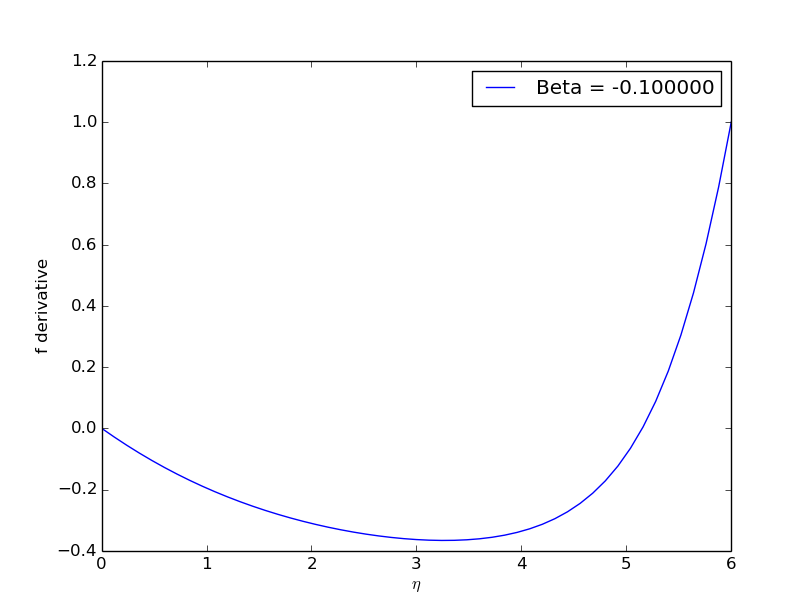
\includegraphics[scale = 0.55]{mand1/fneg.png}
\end{figure}
\begin{figure}[h!]
	\centering
	\caption*{Plot of the h with negative values$\beta$}
	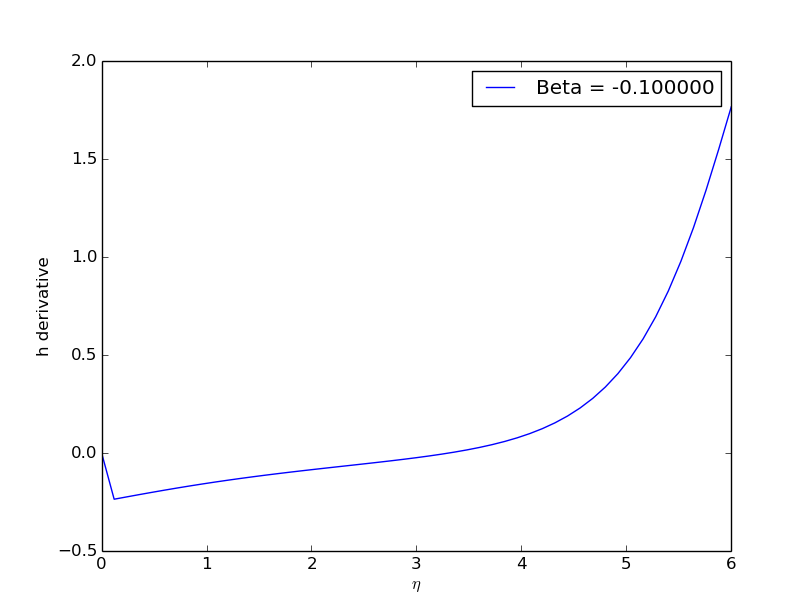
\includegraphics[scale = 0.6]{mand1/hneg.png}
\end{figure}

\newpage
\section{Assignmen II}
In this exercise we are looking at a flow around a cylinder with a circular cross-section. First for a steady flow, then for a time 
dependent flow. I have not succeeded implementing the time dependent flow. \newline
For the steady flow we have the following inflow condition
\begin{align*}
U(0,y) = 4U_my\frac{(H-y)}{H^2}, \hspace{1cm} V = 0
\end{align*}
We are requested to compute the drag/lift coefficients, length of the recirculation zone $L_a$ and the pressure difference $\Delta P$
The coefficients can be calculated the following way.
\begin{align*}
c_D = \frac{2F_w}{\rho \overline{U} D} \hspace{1cm} c_F = \frac{2F_a}{\rho \overline{U} D}
\end{align*}
While $\Delta P$ is defined as $\Delta P = P(x_a,y_a,t) - P(x_e,y_e,t)$, where these to points represent the front and end point of the
cylinder $(x_a,y_a) = (0.15,0.2), (x_b,y_b) = (0.25,0.2) $
Implementing a Falkner-Skan solver for the system, I get the following velocity field and terminal output.
\begin{figure}[h!]	
	\centering
	\caption*{Velocity field $\beta$ }
	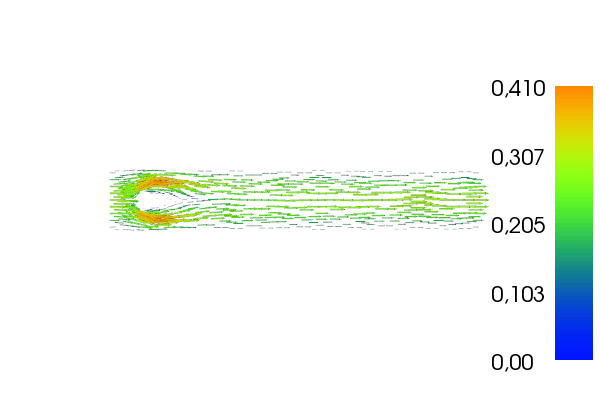
\includegraphics[scale = 0.6]{mand2/velocity.png}
\end{figure}
\begin{lstlisting}[style=terminal]
Calulated values: Cd = 5.234797, Cl = -0.007819 pdiff = 0.014665
\end{lstlisting}
The velocity field seems like a good representation of the flow around the cylinder. We got a faster flow as the fluid passes
the cylinder, and a calmer recirculation zone behind. 


\newpage
\section*{Assignment III}
In this assignment we are looking at a fully developed turbulent channel flow. We are presented with the following
\begin{align*}
0 &= \nu \frac{\partial^2 \bar{u}}{\partial y^2} - \frac{1}{\rho} \frac{\partial \bar{p}}{\partial x} -
\frac{\partial \overline{u^\prime v^\prime}}{\partial y} \\
\overline{u^\prime v^\prime} &= -\nu_t \frac{\partial \bar{u}}{\partial y} \hspace{1cm} \nu_t = l^2
|\frac{\partial \bar{u}}{\partial y}| \hspace{1cm} y^+ = \frac{yv^*}{\nu} = 0 \\
l &= \kappa y \Big(1- \Big(-\frac{y^+}{A} \Big) \Big)
\end{align*}
We start up by using Hint 1, which states that the pressure gradient is constant. We integrate the momentum equation
along the channel. Due to how Hint 2 presents how the mesh can be made, we must take in to account that the mesh is 
reversed, here h is the distance from the wall towards the centre of the channel.

\begin{align*}
\int_0^h \Big(\nu \frac{\partial^2 \bar{u}}{\partial y^2} - \frac{1}{\rho} \frac{\partial \bar{p}}{\partial x} -
\frac{\partial \overline{u^\prime v^\prime}}{\partial y} \Big) dy &=  0\\
\nu \frac{\partial \bar{u}}{\partial y} \Big|^h_0 - \frac{1}{\rho} \frac{\partial \bar{p}}{\partial x}h -
\bar{u}\bar{v}\Big|^h_0 &= 0
\end{align*}
Knowing that $\frac{\partial \bar{u}}{\partial y} = 0$ in the centre, that $l = 0$ for y = 0 and
that $v^* = \sqrt{\nu \frac{\partial \bar{u}}{\partial y}}$ at the wall, we end up with

\begin{align*}
\frac{1}{\rho} \frac{\partial \bar{p}}{\partial x} = - \frac{(v^*)^2}{h}
\end{align*}

Now we have to take a look at the variational form of the problem. It's important to note that the simple v is here a testfunction, not a part of the velocity. Using presented information, and our results from Hint 1 we get the following
\begin{align*}
\int_\Omega l^2\frac{\partial}{\partial y} \frac{\partial \bar{u}}{\partial y} |\frac{\partial u}{\partial y}| v dx 
= -\int_\Omega l^2|\frac{\partial \bar{u}}{\partial y}| \frac{\partial \bar{u}}{\partial y} \frac{\partial v}{\partial y} dx + l^2|\frac{\partial \bar{u}}{\partial y}| \frac{\partial \bar{u}}{\partial y} v \Big|^{\partial \Omega} 
\hspace{1cm} |\frac{\partial \bar{u}}{\partial y}| \frac{\partial \bar{u}}{\partial y} v \Big|^{\partial \Omega} &= 0 \\
\int_\Omega \Big(\nu \frac{\partial^2 \bar{u}}{\partial y^2}v - \frac{1}{\rho} \frac{\partial \bar{p}}{\partial x}v -
\frac{\partial \overline{u^\prime v^\prime}}{\partial y}v  \Big)dx &= 0 \\
\nu\int_\Omega \nabla u \cdot \nabla v dx - \int_\Omega \frac{(v^*)^2}{h} v dx
+ \int_\Omega l^2|\frac{\partial \bar{u}}{\partial y}| \frac{\partial \bar{u}}{\partial y} \frac{\partial v}{\partial y} vdx &= 0
\end{align*}
We make a skewed mesh with high concentration of node points close to the wall, because this is the area we need 
most of our nodes to capture what's going on. Regarding nodes, we are asked how many nodes are needed to ensure 
$y^+ < 1$ by using a regularly spaced mesh. And the answer to that is all too many, which we can't represent on an ordinary computer. With the skewed mesh we get the following result.
\newpage
\begin{figure}[h!]
	\centering
	\caption*{Plot of the numerical solution  }
	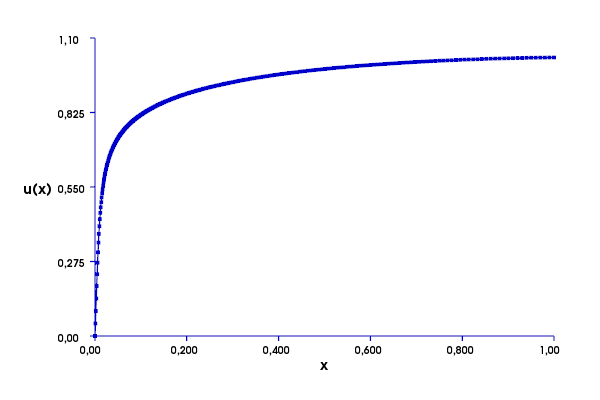
\includegraphics[scale = 0.6]{mand3/numerical.png}

	\caption*{Theoretical result agains numerical problem  }
	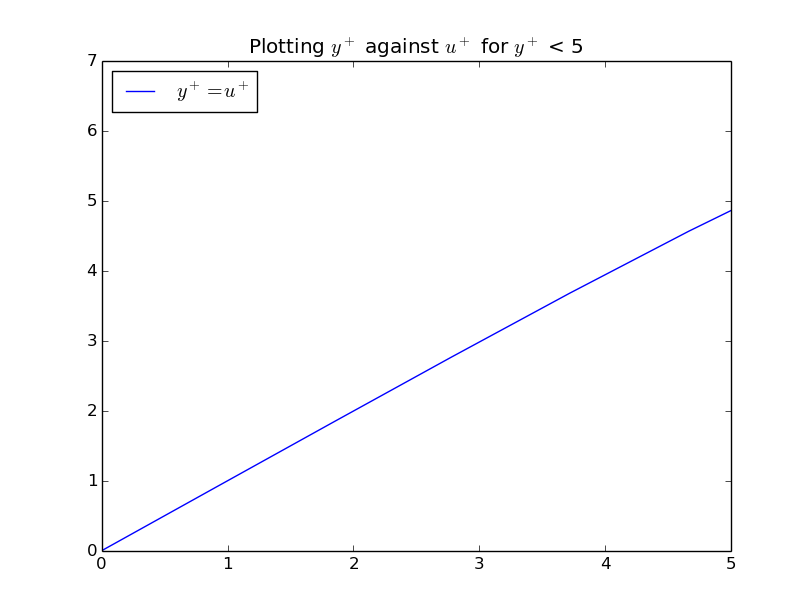
\includegraphics[scale = 0.6]{mand3/linear.png}	
\end{figure}
\newpage
\begin{figure}[h!]
	\centering
	\caption*{Theoretical result agains numerical problem }
	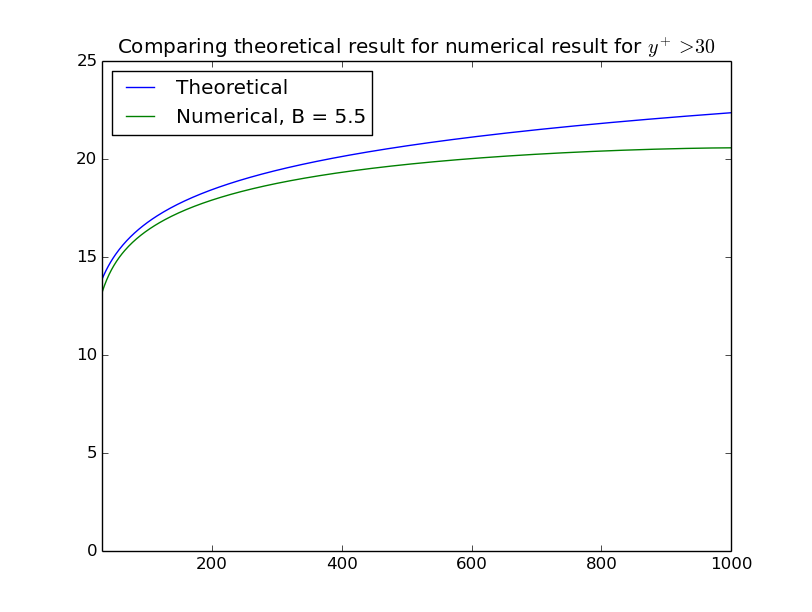
\includegraphics[scale = 0.6]{mand3/theo.png}
\end{figure}

We are supposed to compare our numerical solution to two theoretical results presented in the exercise. 
\begin{align*}
y^+ &= u^+ \hspace{2.3cm} y^+ < 5 \\
u^+ &= \frac{1}{\kappa}ln y^+ + B \hspace{1cm} y^+ > 30 
\end{align*}
Looking at plot number 2, we can see that our numerical solution looks good in terms of the first theoretical 
result. We clearly see linearity in the specified domain. \newline 
For the second theoretical result we see that our numerical results is a good approximation around the wall, but 
falls short as the distance to the wall increases. This is not too surprising due to the theoretical solution is bounded to $y^+ > 30 $. Hence the theoretical and numerical solutions should be closer to each other at the wall.
Calculating the turbulent viscosity at the centre of the channel yields $\nu_t = 0.0011820$. I don't find this value reasonable due to the fact that we know from experiments that alot of turbulence occur at that particular area, so the numerical result and experiments differ.


\newpage
\section*{Assignment IV}

\begin{itemize}
\item{} Reynolds Averaged Navier Stokes equations \newline
We start the derivation with our base, the Navier Stokes equations \newline
Defining a velocity field  $\mathbf{v} = (u,v,w) = (u_1, u_2, u_3)$ \newline
We now express the velocity components as a sum of their mean value and their corresponding fluctuation
$u =\bar{u} + u^\prime, v =\bar{v} + v^\prime, w =\bar{w} + w^\prime$ by direct insertion 

\begin{align*}
\nabla \cdot \mathbf{V} &= \frac{\partial u_i}{\partial x_i} = 0 \\
\rho \frac{D\mathbf{v}}{Dt} &= \rho \frac{Du_i}{Dt} =
- \frac{\partial p}{\partial x_i} + \mu \frac{\partial^2 u_i}{\partial x_j \partial x_j} 
\end{align*}
\begin{align*}
\frac{\partial(\bar{u}_i + u^\prime_i)}{\partial x_i} &= 0 \\
\rho \frac{D(\bar{u}_i + u^\prime_i)}{Dt} &= \rho\big(\frac{\partial(\bar{u}_i + u^\prime_i)}{\partial t}   
+ (\bar{u}_j + u^\prime_j) \frac{\partial (\bar{u}_i + u^\prime_i)}{\partial x_j} \big) =
- \frac{\partial (\bar{p} + p^\prime)}{\partial x_i} + \mu \frac{\partial^2(\bar{u}_i + u^\prime_i)}
{\partial x_j \partial x_j}
\end{align*}

We observe that the convective term can be rewritten, and that the last term is zero due to the
continuum equation.
 
\begin{align*}
(\bar{u}_j + u^\prime_j) \frac{\partial (\bar{u}_i + u^\prime_i)}{\partial x_j} &= 
\frac{\partial (\bar{u}_i + u^\prime_i)(\bar{u}_j + u^\prime_j)}{\partial x_j} -
(\bar{u}_i + u^\prime_i)\frac{\partial (\bar{u}_j + u^\prime_j)}{\partial x_j} \\
\rho\big(\frac{\partial(\bar{u}_i + u^\prime_i)}{\partial t}   
+   \frac{\partial (\bar{u}_i + u^\prime_i)(\bar{u}_j + u^\prime_j)}{\partial x_j} &=
- \frac{\partial (\bar{p} + p^\prime)}{\partial x_i} + \mu \frac{\partial^2(\bar{u}_i + u^\prime_i)}
{\partial x_j \partial x_j}
\end{align*}
We know time-average the whole equation, getting rid of some of the terms and we end up with the following result

\begin{align*}
\rho \big( \frac{\partial \bar{u}_i}{\partial t} + \frac{\bar{u_i}\bar{u_j}}{\partial x_j} 
+ \frac{\partial \overline{u^\prime_i u^\prime_j}}{\partial x_j}  \big) = 
- \frac{\partial \bar{p}}{\partial x_i} + \mu \frac{\partial^2 \bar{u}_i}{\partial x_j \partial x_j}
\end{align*}
To help out making the equation more compact, we apply the chain rule on the mean convection part, and yet again
observing that the last term is zero due to our continuum relation. We end up with the final result

\begin{align*}
\frac{\bar{u_i}\bar{u_j}}{\partial x_j} = \frac{\bar{u}_j \partial \bar{u}_i}{\partial x_j} +
 \frac{\bar{u}_i \partial \bar{u}_j}{\partial x_j} = \frac{\bar{u}_j \partial \bar{u}_i}{\partial x_j} \\
\rho \big( \frac{\partial \bar{u}_i}{\partial t} +  \frac{\bar{u}_j \partial \bar{u}_i}{\partial x_j} \big) = 
- \frac{\partial \bar{p}}{\partial x_i} + \frac{\partial}{\partial x_j}
\big(\mu \frac{\bar{u}_i}{\partial x_j} - \rho \overline{u^\prime_i u^\prime_j}  \big)
\end{align*}
\newpage
\item{} The Turbulence Kinetic-Energy Equation \newline
We use the same notations and defined velocity fields in this derivation. We start up with the substituted
Navier Stokes equations, but this time we multiply them by $u^\prime$

\begin{align*}
u^\prime_i \big(\frac{\partial(\bar{u}_i + u^\prime_i)}{\partial t}
+ (\bar{u}_j + u^\prime_j) \frac{\partial (\bar{u}_i + u^\prime_i)}{\partial x_j} \big) =
- \frac{u^\prime_i}{\rho}\frac{\partial (\bar{p} + p^\prime)}{\partial x_i} + \nu u^\prime_i  
\frac{\partial^2(\bar{u}_i + u^\prime_i)} {\partial x_\partial x_j}
\end{align*}
Time averaging the equation, we will continue manipulating the terms in the x-direction to easier 
see what's going on

\begin{align*}
\overline{u^\prime \frac{\partial u^\prime}{\partial t}} + \bar{u}\overline{u^\prime \frac{\partial u^\prime}
{\partial x}} + \overline{u^{\prime 2}\frac{\partial u^\prime}{\partial x}} + \bar{v} 
\overline{u^\prime \frac{\partial u^\prime}{\partial y}} + \overline{u^\prime v^\prime}\frac{\partial \bar{u}}
{\partial y} + \overline{u^\prime v^\prime \frac{\partial u^\prime}{\partial y}} + \bar{w}\overline{u^\prime	
\frac{\partial u^\prime}{\partial z}} + \overline{u^\prime w^\prime} \frac{\partial \bar{u}}{\partial z} + \\
\overline{u^\prime w^\prime \frac{\partial u^\prime}{\partial z}} = - \overline{\frac{u^\prime}{\rho} 
\frac{\partial p^\prime}{\partial x}} + \nu \overline{u^\prime \big(\frac{\partial ^2 u^\prime}{\partial x^2} +
\frac{\partial ^2 u^\prime}{\partial y^2} + \frac{\partial ^2 u^\prime}{\partial z^2}\big)}
\end{align*}
The next step is to rewrite the left hand side of the equation. We do this to aquire a similar form to kinetic energy.

\begin{align*}
\frac{1}{2} \frac{\partial \overline{u^{\prime 2}}}{\partial t} + \bar{u}\frac{1}{2} \frac{\partial \overline{
u^{\prime2}}}{\partial x} + \bar{v}\frac{1}{2}\frac{\partial \overline{u^{\prime2}}}{\partial y} + 
\bar{w}\frac{1}{2}\frac{\partial \overline{u^{\prime2}}}{\partial z} + \overline{u^{\prime 2}} 
\frac{\partial \bar{u}}{\partial x} + \overline{u^\prime v^\prime} \frac{\partial \bar{u}}{\partial y} + 
\overline{u^\prime w^\prime} \frac{\partial \bar{u}}{\partial z} + \\ \Big[
 \overline{u^{\prime 2} \frac{\partial u^\prime}{\partial x}} +  \overline{u^\prime v^\prime \frac{\partial u^\prime}{\partial y}} +  \overline{u^\prime w^\prime \frac{\partial u^\prime}{\partial z}} \Big]  
\end{align*}
The last term marked in brackets can be rewritten, and by using continuity term, the system can be written as

\begin{align*}
\frac{1}{2} \frac{\partial \overline{u^{\prime 2}}}{\partial t} + \bar{u}\frac{1}{2} \frac{\partial \overline{
u^{\prime2}}}{\partial x} + \bar{v}\frac{1}{2}\frac{\partial \overline{u^{\prime2}}}{\partial y} + 
\bar{w}\frac{1}{2}\frac{\partial \overline{u^{\prime2}}}{\partial z} = -\overline{u^{\prime 2}} 
\frac{\partial \bar{u}}{\partial x} - \overline{u^\prime v^\prime} \frac{\partial \bar{u}}{\partial y} - 
\overline{u^\prime w^\prime} \frac{\partial \bar{u}}{\partial z} \\
-\overline{\frac{u^\prime}{\rho} \frac{\partial p^\prime}{\partial x}} - \frac{1}{2}\Big[\frac{\partial 
\overline{u^{\prime 3}}}{\partial x} + \frac{\overline{u^{\prime 2}v^\prime}}{\partial y} +
\frac{\partial \overline{u^{\prime 2}w^\prime}}{\partial z}  \Big] \ + \nu \overline{u^\prime \nabla^2 u^\prime}
\end{align*} 


By using the exact same approach for the v and w component of $\mathbf{v}$, we end up with similar results. This will turn into something long and nasty, so we will do two things to make the equation more compact. First we define
$K = \frac{1}{2}(\overline{u^\prime u^\prime}+\overline{v^\prime v^\prime}+\overline{w^\prime w^\prime})$. Second we add up the components and by using index notation we get a more pleasant equation to look at.

\begin{align*}
\frac{DK}{Dt} = -\frac{\partial}{\partial x_i} \Big[\overline{ u^\prime_i (\frac{1}{2}u^\prime_j u^\prime_j + \frac{p^\prime}{\rho} ) }\Big] - \overline{u^\prime_i u^\prime_j} \frac{\partial \bar{u_j}}{\partial x_i} +
\frac{\partial}{\partial x_i} \Big[\nu u^\prime_j \Big(\frac{\partial u^\prime_i}{\partial x_j} +
\frac{\partial u^\prime_j}{\partial x_i} \Big) \Big] - \nu \overline{\frac{\partial u^\prime_j}{\partial x_i} 
\Big(\frac{\partial u^\prime_i}{\partial x_j} + \frac{\partial u^\prime_j}{\partial x_i} \Big)}
\end{align*}

\end{itemize}

\newpage 
\section*{Code appendix}
\section*{Exercise I}
\lstinputlisting[style=python]{mand1/mand1.py}  
\newpage
\section*{Exercise II}
\lstinputlisting[style=python]{mand2/mand22.py}  
\newpage
\section*{Exercise III}
\lstinputlisting[style=python]{mand3/mand3.py}  



\end{document}

